\chapter{Evaluation and benchmarks}
In this chapter we first evaluate both the correctness of our code generator,
and the performance of the \csharp{} programs that our code generator generates.
For testing correctness, we use the Futhark compiler's existing test suite with
our new code generator. For the performance evaluation, we , we run and compare benchmark
results between programs generated by the Futhark \csharp{}-, \C{}- and \Python{} code generators.

We then evaluate whether the \fshark{} language succeeds in letting us write
complex GPU benchmarks in an idiomatic \fsharp{} style.

Finally, we evaluate the \fshark{} compiler itself. First we test whether the
\fshark{} compiler correctly translates \fshark{} programs to Futhark, so that
they are functionally equivalent.
We then compile and compare the performance of GPU benchmarks written in
\fshark{} with equivalent benchmarks written in Futhark.


\section{Correctness of the Futhark csharp{} generator}
\label{subsec:futharkcsharpcorrectness}
To show that the Futhark \csharp{} code generator correctly translates Futhark
to \csharp{} programs, we have chosen to test our solution using the already existing Futhark test
suite.

The Futhark test suite is located in the folder \texttt{./tests} in the Futhark
repository. For our evalutations, we first apply the test suite to our \csharp{}
code generator for non-OpenCL programs using the following command from the
Futhark root folder:

\begin{minted}{bash}
$ futhark-test --compiler=futhark-cs tests/
\end{minted}

Then, we apply the test suite on our code generator for \csharp{} OpenCL
programs, like so:

\begin{minted}{bash}
$ futhark-test --compiler=futhark-csopencl tests/
\end{minted}



\section{The performance of Futhark \csharp{} programs}
\label{subsec:futharkcsharpperformance}
To determine whether Futhark \csharp{} programs have similar performance to
Futhark C and Futhark Python programs, we have used Futhark's own benchmark
suite.
Using this benchmark suite, we have compared the runtime of over 30 different
benchmarks when executed as \csharp{}-, C- and Python Futhark OpenCL programs
respectively.

HOW CAN THEY BE RUN



\section{The design of the \fshark{} language}
\label{sec:fsharklanguageeval}
One of the goals of \fshark{} is to enable users to write complex GPU programs
using idiomatic \fsharp{} code.

To test this, we have taken two already existing benchmark implementations from
Futhark, and manually translated them to \fshark{}.

\subsection{LocVolCalib}
First, we present the \fshark{} version of the LocVolCalib (respectively
FSharpTests/Benchmarks/LocVolCalib.fs and finpar/LocVolCalib.fut in the
\fshark{} and Futhark benchmarks repository.) from the Finpar\cite{finpar}
benchmark suite.

We have chosen this benchmark as it is features plenty of nested SOACs, and is
in general a structurally complex program.

Below, we show multiple snippets of the \fshark{} and Futhark version of the
LocVolCalib benchmark to demonstrate
\begin{minted}[fontsize=\scriptsize, breaklines]{fsharp}
;; Snippet from FShark's LocVolCalib
let explicitMethod (myD:    float32 [] []) (myDD: float32 [] [])
                   (myMu:   float32 [] []) (myVar: float32 [] [])
                   (result: float32 [] [])
                  : float32 [] [] =
  // 0 <= i < m AND 0 <= j < n
  let m = Length myDD
  Map3 (fun (mu_row : float32 []) (var_row : float32 []) (result_row : float32 []) ->
    Map5 (fun (dx : float32 []) (dxx : float32 []) (mu : float32) (var : float32) (j : int) ->
      let c1 = if 0 < j
               then (mu*dx.[0] + 0.5f*var*dxx.[0]) * result_row.[j-1]
               else 0.0f
      let c3 = if j < (m-1)
               then (mu*dx.[2] + 0.5f*var*dxx.[2]) * result_row.[j+1]
               else 0.0f
      let c2 = (mu*dx.[1] + 0.5f*var*dxx.[1]) * result_row.[j]
      in  c1 + c2 + c3) myD myDD mu_row var_row <| (Iota m)
   ) myMu myVar result

// for implicitY: should be called with transpose(u) instead of u
let implicitMethod (myD:  float32 [] [])  (myDD:  float32 [] [])
                   (myMu: float32 [] [])  (myVar: float32 [] [])
                   (u:    float32 [] [])  (dtInv: float32)
                    : float32 [] [] =
  Map3 (fun (mu_row : float32 []) (var_row : float32 []) (u_row : float32 []) ->
    let (a,b,c) = Unzip3 (
      Map4 (fun (mu : float32) (var : float32) (d : float32 []) (dd : float32 []) ->
        (0.0f - 0.5f*(mu*d.[0] + 0.5f*var*dd.[0]), dtInv - 0.5f*(mu*d.[1] + 0.5f*var*dd.[1]), 
        0.0f   - 0.5f*(mu*d.[2] + 0.5f*var*dd.[2])
        )
      ) mu_row var_row myD myDD
    )
    in tridagPar a b c u_row
  ) myMu myVar u
\end{minted}

\begin{lstlisting}[language=Futhark]
-- Snippet from Futhark's LocVolCalib
let explicitMethod [m][n] (myD:    [m][3]f32,  myDD: [m][3]f32,
                           myMu:   [n][m]f32,  myVar: [n][m]f32,
                           result: [n][m]f32)
                  : *[n][m]f32 =
  -- 0 <= i < m AND 0 <= j < n
  map3 (\mu_row var_row result_row ->
    map5 (\dx dxx mu var j ->
      let c1 = if 0 < j
               then (mu*dx[0] + 0.5*var*dxx[0]) * unsafe result_row[j-1]
               else 0.0
      let c3 = if j < (m-1)
               then (mu*dx[2] + 0.5*var*dxx[2]) * unsafe result_row[j+1]
               else 0.0
      let c2 =      (mu*dx[1] + 0.5*var*dxx[1]) * unsafe result_row[j  ]
      in  c1 + c2 + c3) myD myDD mu_row var_row (iota m)
  ) myMu myVar result

-- for implicitY: should be called with transpose(u) instead of u
let implicitMethod [n][m] (myD:  [m][3]f32,  myDD:  [m][3]f32,
                           myMu: [n][m]f32,  myVar: [n][m]f32,
                           u:   *[n][m]f32,  dtInv: f32)
                  : *[n][m]f32 =
  map3 (\mu_row var_row u_row  ->
    let (a,b,c) = unzip3 
      (map4 (\mu var d dd ->
        ( 0.0   - 0.5*(mu*d[0] + 0.5*var*dd[0])
        , dtInv - 0.5*(mu*d[1] + 0.5*var*dd[1])
        , 0.0   - 0.5*(mu*d[2] + 0.5*var*dd[2]))
      ) mu_row var_row myD myDD)
    in tridagSeq (a, copy b, c, copy u_row )
  myMu myVar u
\end{lstlisting}
There are a couple of differences. The Futhark version can define the lengths of
the dimensions of its arrays in the function definition. These lengths can then
be used as variables in the function body. An example of this is shown in the
Futhark example: At line 2 we define that our input arrays have $n*m$ elements,
or in some cases $3*m$, and we can then use these lengths, such as in the
if-expression on line 12.

The second difference is on line 31 of the Futhark version. Here, we copy the
array used for our function call, which is a feature used for Futhark's
uniqueness types\cite{uniqueness}.
As we don't have uniqueness types in \fshark{}, we can leave out this copy in
the \fshark{} version, as shown in line 33.

The third difference is the usage of the \texttt{unsafe} expression in Futhark's
example at line 10, 13 and 15. We need them in Futhark to circumvent Futhark's
boundary checks for array indexing, but we can leave them out in the \fshark{}
version, as \fshark{} doesn't have that kind of boundary checks.

The second pair of snippets are shown below.

\begin{minted}{fsharp}
let value (numX: int) (numY: int) (numT: int) (s0: float32) (strike: float32) (t: float32) (alpha: float32) (nu: float32) (beta: float32): float32 =
  let (myXindex, myYindex, myX, myY, myTimeline) = initGrid s0 alpha nu t numX numY numT
  let (myDx, myDxx) = initOperator myX
  let (myDy, myDyy) = initOperator myY
  let myResult = setPayoff strike myX myY
  let myTimeline_neighbours = Reverse (Zip (Init myTimeline) (Tail myTimeline))

  let myResult' = 
    Foldl (fun oldResult (tnow,tnext) ->
      let (myMuX, myVarX, myMuY, myVarY) =
        updateParams myX myY tnow alpha beta nu
      in rollback tnow tnext oldResult
            myMuX myDx myDxx myVarX
            myMuY myDy myDyy myVarY
      ) myResult myTimeline_neighbours
  in myResult'.[myYindex].[myXindex]
\end{minted}

\begin{lstlisting}[language=Futhark]
let value(numX: i32, numY: i32, numT: i32, s0: f32, strike: f32, t: f32, alpha: f32, nu: f32, beta: f32): f32 =
  let (myXindex, myYindex, myX, myY, myTimeline) =
    initGrid(s0, alpha, nu, t, numX, numY, numT)
  let (myDx, myDxx) = initOperator(myX)
  let (myDy, myDyy) = initOperator(myY)
  let myResult = setPayoff(strike, myX, myY)
  let myTimeline_neighbours = reverse (zip (init myTimeline) (tail myTimeline))

  let myResult = loop (myResult) for (tnow,tnext) in myTimeline_neighbours do
      let (myMuX, myVarX, myMuY, myVarY) =
        updateParams(myX, myY, tnow, alpha, beta, nu)
      let myResult = rollback(tnow, tnext, myResult,
                              myMuX, myDx, myDxx, myVarX,
                              myMuY, myDy, myDyy, myVarY)

      in myResult
  in myResult[myYindex,myXindex]
\end{lstlisting}
There are two major differences: First, the \fshark{} version doesn't take one
single tuple as the function argument, but does instead need to take the tuple
elements as arguments individually. This is because of the \fsharp{} compiler's
currying, as described in section~\ref{noteonfsharktypes}.

Second, we have translated the Futhark version's for loop on line 9 into a
\texttt{Foldl} on line 9 of the \fshark{} version. This is because the current
version of \fshark{} doesn't support \texttt{for-loops}.
Otherwise, the two expressions are equivalent.

The complete \fshark{} version is available in
appendix~\ref{app:fsharklocvolcalib}, with the Futhark version available in
appendix~\ref{app:futharklocvolcalib} for reference.

\subsection{nbody}













\section{The usability and design of the \fshark{} language}

\subsection{The correctness of the \fshark{} subset.}
\label{subsec:fsharkcorrectness}
When transpiling code from one language to another, it is absolutely vital that
the programmer can trust that the target language result
is semantically equivalent to the source language code.

In \fshark{}s case, it means that any program written using the \fshark{}
subset must have the same result no matter whether it is run natively as
\fsharp{} code, or run as \fshark{} compiled Futhark code.

Take for example the logarithm function \texttt{log}. In both \fsharp{} and
Futhark, this function denotes the natural logarithm. If we were translating
from a careless language $l$, where \texttt{log} instead denoted the binary
logarithm, the translation would still be succesfull and not trigger any type
errors.
However, the native result and the Futhark result would be wildly different.

To ensure that every operator and function in the \fshark{} subset has
equivalent results, no matter whether the \fshark{} code is run as native
\fsharp{} code, or compiled into Futhark, I have written a test suite with unit
tests for each element in the \fsharp{} subset. 

An \fshark{} test is an \fshark{} module, but with two extra values added,
namely an input and an output value for the test. For example, the test written for the
division operator is shown in figure \ref{fig:fsharkdivtest}.

\begin{figure}[h]
  \centering
\begin{minted}[breaklines=true, fontsize=\footnotesize]{fsharp}
module Div
open FSharkPrelude.FSharkPrelude
open FShark.TestTypes.TestTypes
open System

[<FSharkEntry>]
let div (fiveByte : int8) (fiveShort : int16) (five : int) 
        (fiveLong : int64) (fiveSingle : single) (fiveDouble : double) 
        : (int8 * int16 * int * int64 * single * double) =

    (fiveByte / 2y, fiveShort / 2s, five / 2, 
     fiveLong / 2L, fiveSingle / 2.0f, fiveDouble / 2.0)

[<FSharkInput>]
let value = [|5y; 5s; 5; 5L; 5.0f; 5.0|] : obj array

[<FSharkOutput>]
let sameValue = 
  (2y, 2s, 2, 2L, 2.5f, 2.5) : (int8 * int16 * int * int64 * single * double)
\end{minted}
  \caption{The unit test for the \fshark{} division operator}
  \label{fig:fsharkdivtest}
\end{figure}
\subsection{Correctness of \fshark{} translations }
- tested by comprehensive suite of unit tests
\subsubsection{Testing arithmetic operators}
For all arithmetic operators available in \fshark{}, I have written an
accompanying test, suitably located in the directory
\texttt{FSharkTests/UnitTests/Operators} in the \fshark{} project.

The test suite for the operators are quite rudimentary, and are primarily
designed to confirm that the types of the operands are preserved when passed to
Futhark \csharp{} and back again.

The test suite does not test edges (such as integer overflows or dividing
decimals by zero) behaves equally in natively executed \fshark{} code and
translated Futhark \csharp{} code.
These edge cases has been left out for SOME reasons.

(THESE ARE NOT ACTUALLY DONE YET)
(Are unit tests enough?)

all convertion functions pass through i64. this might be a mistake, as real
supports f32 to f64

thoughts on correctness of translations
testing correctness of these translations

\subsubsection*{Testing \fsharp{} standard library functions}

\subsubsection*{On comparing floating point values}


\subsection{Evaluating the \fshark{} language design}
- compare benchmarks written in \fshark{} with benchmarks written in Futhark.



\section{The performance of \fshark{} generated GPU kernels}
\label{sec:fsharkgpubenchmarks}

Appendices show 
\section*{The \texttt{LocVolCalib} benchmark}
small.in:
FShark (openCL) took 211882 microseconds.
Average invokation (fshark non openCL) time was 81194767 microseconds.
Native took 438 929 311 microseconds.

\begin{figure}
    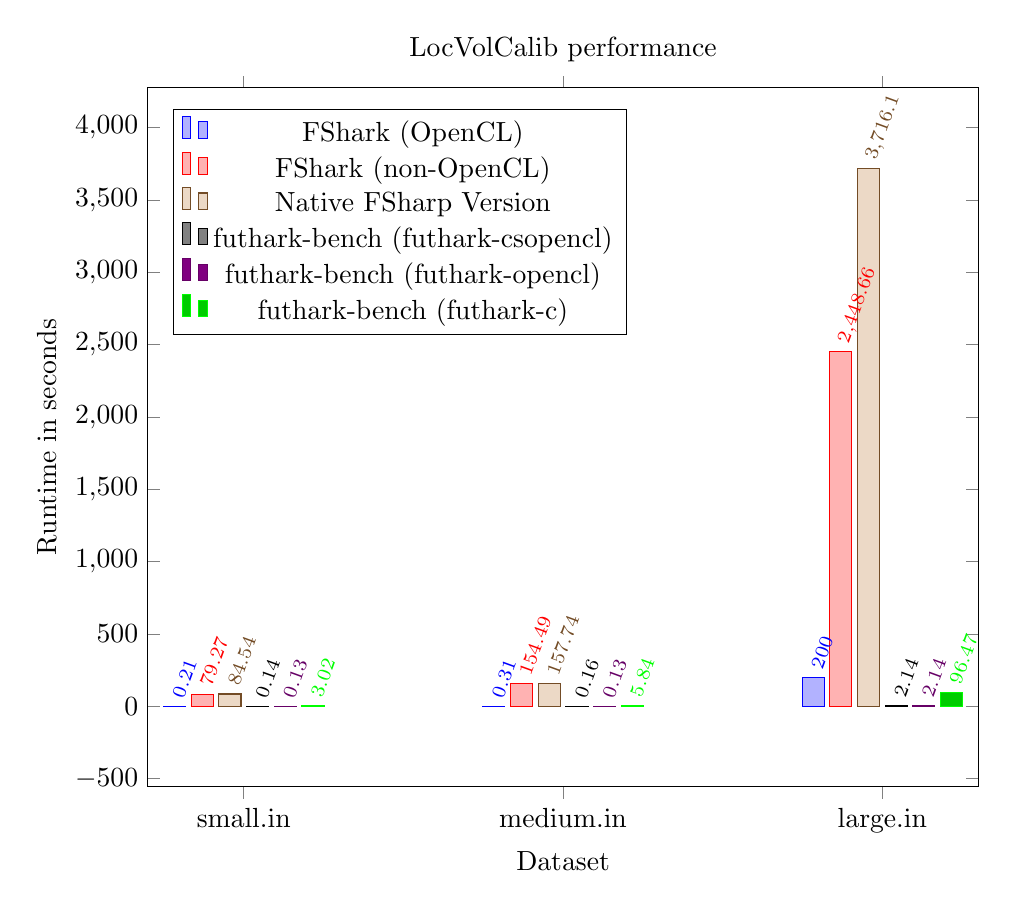
\begin{tikzpicture}
      \begin{axis}[
        title={LocVolCalib performance},
        xlabel={Dataset},
        ylabel={Runtime in seconds},
        width=1\textwidth,
        %height=0.5,
        symbolic x coords={small.in,medium.in,large.in},
        xtick=data,
        enlargelimits=0.15,
        ybar=2pt,% configures ‘bar shift’
        bar width=8pt,
        nodes near coords,
        every node near coord/.append style={rotate=70, anchor=west,font=\scriptsize},
        legend style={legend pos=north west}
      ]
      \addplot plot coordinates {(small.in, 0.21 ) (medium.in, 0.31 ) (large.in, 200.0 )};
      \addplot plot coordinates {(small.in, 79.265 ) (medium.in, 154.488 ) (large.in, 2448.660 )};
      \addplot plot coordinates {(small.in, 84.537 ) (medium.in, 157.735 ) (large.in, 3716.097 )};
      \addplot plot coordinates {(small.in, 0.14 ) (medium.in, 0.16 ) (large.in, 2.14 )};
      \addplot plot coordinates {(small.in, 0.13 ) (medium.in, 0.13 ) (large.in, 2.14 )};
      \addplot plot coordinates {(small.in, 3.02 ) (medium.in, 5.84 ) (large.in, 96.47 )};

      \legend{FShark (OpenCL), FShark (non-OpenCL), Native FSharp Version, futhark-bench (futhark-csopencl), futhark-bench (futhark-opencl), futhark-bench (futhark-c)}
      \end{axis}
    \end{tikzpicture}
    \caption{Comparison between Python and Futhark performance for simple model}
    \label{fig:line-graph}
\end{figure}

medium.in:
(Fshark opencl)invokation time was 310833 microseconds
Fshark nonopencl Average invokation time was 154 141 321 ms
Native took 900 643005 microseconds.

large.in:

fshark with opencl Memory Allocation Error
fshark sans opencl 2450 637 053 microseconds
Native took 24757 874 577 microseconds.


for all three datasets
%% master ●  futhark-bench --compiler=futhark-csopencl LocVolCalib.fut 
%%Compiling LocVolCalib.fut...
%%Results for LocVolCalib.fut:
%dataset LocVolCalib-data/small.in:   143015.70us (avg. of 10 runs; RSD: 0.02)
%dataset LocVolCalib-data/medium.in:  143581.70us (avg. of 10 runs; RSD: 0.00)
%dataset LocVolCalib-data/large.in:  1987195.20us (avg. of 10 runs; RSD: 0.00)
%%
%% master ●  futhark-bench --compiler=futhark-opencl LocVolCalib.fut 
%%Compiling LocVolCalib.fut...
%%Results for LocVolCalib.fut:
%%dataset LocVolCalib-data/small.in:   134473.30us (avg. of 10 runs; RSD: 0.02)
%%dataset LocVolCalib-data/medium.in:  134796.20us (avg. of 10 runs; RSD: 0.01)
%%dataset LocVolCalib-data/large.in:  1924412.20us (avg. of 10 runs; RSD: 0.01)

%% master ●  futhark-bench --compiler=futhark-c LocVolCalib.fut     
%%Compiling LocVolCalib.fut...
%%Results for LocVolCalib.fut:
%%dataset LocVolCalib-data/small.in:  3 020588.60us (avg. of 10 runs; RSD: 0.01)
%%dataset LocVolCalib-data/medium.in: 5 842482.00us (avg. of 10 runs; RSD: 0.01)
%%dataset LocVolCalib-data/large.in:  96 476520.00us (avg. of 10 runs; RSD: 0.00)
%%


\section*{The \texttt{nbody} benchmark}

for all three datasets


\subsection*{Specifications for benchmark}
We have run the benchmarks on a system with these attributes:
\begin{itemize}
\item CPU: 4 cores of Intel Core i5-6500 at 3.20GHz
  \begin{itemize}
  \item L1 cache: 128 KiB 
  \item L2 cache: 1024 KiB 
  \item L3 cache: 6144 KiB 
  \end{itemize}
\item GPU: GeForce GTX 970
\end{itemize}


Introduction for the two benchmarks LocVolCalib and nbody



why are they faster in general




%%% Local Variables:
%%% mode: latex
%%% TeX-master: "../thesis"
%%% End: